\documentclass[12pt]{report}

% ---- Packages ----
\usepackage[utf8]{inputenc}
\usepackage[T1]{fontenc}
\usepackage{graphicx}
\usepackage{geometry}
\geometry{margin=1in}
\usepackage{setspace}
\usepackage{titling}

% ---- Metadata ----
\title{\Huge Desert Tortoise Network Analysis\\[1ex]
        \large Social Network Analysis – PR1}
\author{Diego Monroy Minero\\[0.5ex]Universidad Politécnica de Yucatán}
\date{\textbf{Delivery Date:} June 22, 2025}

% ---- Document ----
\begin{document}

% -- Title Page --
\begin{titlepage}
    \thispagestyle{empty}
    \begin{center}
        \vspace*{2cm}
        % Logo
        
\includegraphics[width=0.35\textwidth]{Images/Logo UPY.png}\\[2cm]
        % Title block
        {\Huge \textbf{Desert Tortoise Network Analysis}}\\[1.5ex]
        {\Large Social Network Analysis – PR1}\\[2cm]
        % Author and institution
        {\Large Diego Monroy Minero}\\[0.5ex]
        {\large Universidad Politécnica de Yucatán}\\[0.5ex]
        {\large Data Science Major}\\[0.5ex]
        {\large 8th Quarter}\\[1.5cm]
        % Professor
        {\large \textbf{Professor:} Didier Gamboa}\\[2cm]
        % Date
        {\Large \textbf{Delivery Date:} June 22, 2025}\\
    \end{center}
    \vfill
    \begin{center}
        \large\textit{“Analyzing social structure in a seemingly solitary species”}
    \end{center}
\end{titlepage}

% -- Abstract --
\begin{abstract}
This report presents a network analysis of the desert tortoise (\textit{Gopherus agassizii}) social structure, based on burrow-sharing data collected over four years (1996–1999) in Nevada, USA. Although the species is generally described as solitary, the analysis reveals non-random social structures emerging from shared refuge use.

Through the application of graph theory and community detection techniques, I identified a moderately sparse but highly clustered undirected network with clear modular organization. Degree, betweenness, and closeness centralities highlighted key individuals acting as hubs or bridges between subgroups. The degree distribution showed a heavy-tailed pattern, and eight distinct communities were detected with a high modularity score (0.5568).

A temporal breakdown showed that the network's structure evolved over time, with clustering increasing and a strong core component forming in 1997–1998. These results suggest that tortoise interactions are influenced by spatial dynamics and habitat reuse, offering insights into the emergent social behavior of a traditionally solitary reptile.
\end{abstract}

% -- Introduction --
\chapter*{Introduction}
\addcontentsline{toc}{chapter}{Introduction}

The dataset analyzed in this report corresponds to the \textit{reptilia-tortoise-network-bsv}, a real-world social network derived from burrow-sharing interactions among desert tortoises (\textit{Gopherus agassizii}). The data was collected in Nevada, USA over a four-year period using radio tagging techniques. The network was first constructed as a bipartite graph, linking tortoises to the burrows they occupied. From this bipartite structure, a projected social network was obtained, where an undirected edge between two tortoises indicates that they used the same burrow, potentially at different times.

This network was previously used in the study by Sah et al. (2016), which aimed to infer social structure in a species generally regarded as solitary. The dataset is particularly important because it challenges the assumption that solitary species do not exhibit structured interaction patterns. By leveraging graph theory, it becomes possible to uncover hidden social dynamics, identify central individuals, and detect communities that emerge from spatial and behavioral interactions.

The network can be classified as:
\begin{itemize}
    \item \textbf{Undirected:} Edges represent mutual burrow usage, with no directionality.
    \item \textbf{Unweighted:} No frequency or intensity of interaction is encoded.
    \item \textbf{Projected from bipartite:} Derived from a bipartite tortoise-burrow graph.
\end{itemize}

A visualization of the full network using a force-directed (spring) layout reveals a moderately sparse structure with distinct dense regions. These regions suggest the presence of subgroups that are further analyzed through community detection. Nodes with high degree and centrality measures stand out as potentially influential individuals, possibly occupying high-use burrows or acting as spatial bridges.

Given the network's ecological context and structural properties, this analysis not only explores theoretical concepts from graph theory (such as clustering, shortest paths, and modularity), but also provides insight into the real-world behavioral patterns of desert tortoises. The results can inform future studies on solitary animal behavior, spatial ecology, and the role of shared resources in shaping social structure.

% -- Network Characteristics --
\chapter*{Network Characteristics}
\addcontentsline{toc}{chapter}{Network Characteristics}

To begin the structural analysis of the tortoise network, several key graph metrics were computed using standard functions from the NetworkX library in Python. These include the network size, density, clustering coefficient, and path-based measurements such as shortest path length, diameter, radius, and eccentricity.

\section*{General Visualization}
Figure~\ref{fig:network-overview} shows a force-directed layout of the full network. The structure is visually sparse but exhibits regions with dense interconnections, suggesting the presence of localized interaction clusters.

\begin{figure}[h!]
    \centering
    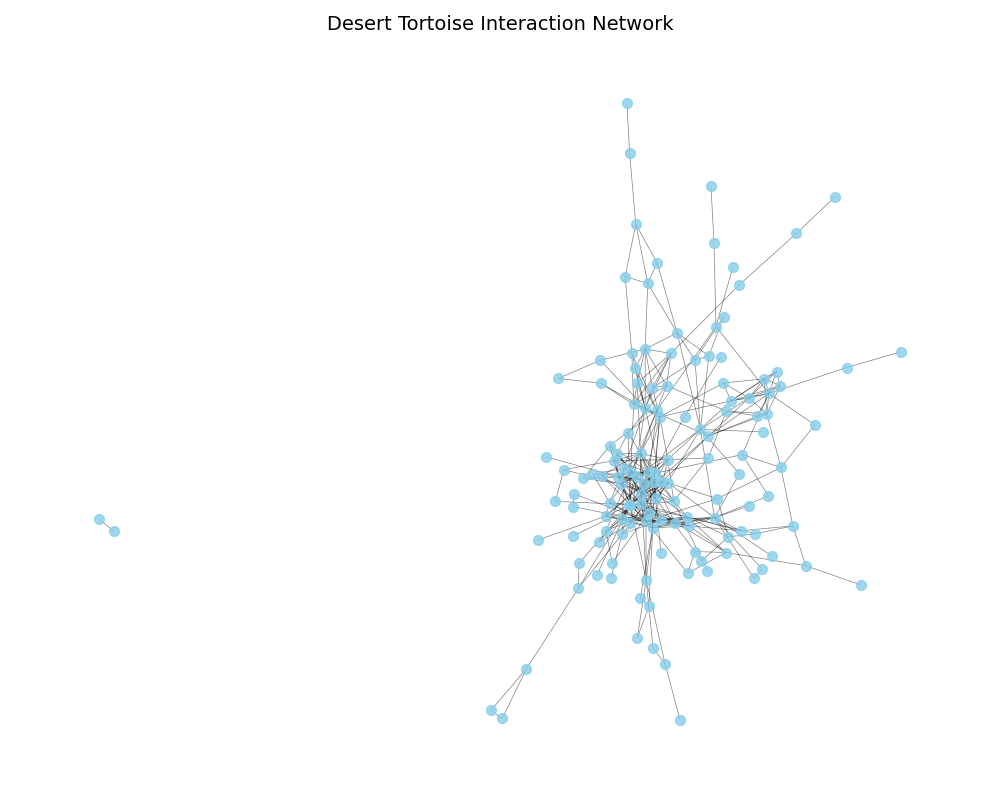
\includegraphics[width=0.8\textwidth]{Images/General Network Visualization.png}
    \caption{Visualization of the tortoise network using spring layout.}
    \label{fig:network-overview}
\end{figure}

\section*{Descriptive Statistics}

The table below summarizes the main structural properties of the full network and its largest connected component.

\begin{table}[h!]
    \centering
    \begin{tabular}{|l|c|}
        \hline
        \textbf{Metric} & \textbf{Value} \\\hline
        Number of nodes & 136 \\\hline
        Number of edges & 374 \\\hline
        Network density & 0.0407 \\\hline
        Average degree & 5.50 \\\hline
        Minimum degree & 1 \\\hline
        Maximum degree & 19 \\\hline
        Average clustering coefficient & 0.3335 \\\hline
        Number of connected components & 2 \\\hline
        Size of largest connected component & 134 nodes \\\hline
        Average shortest path length (LCC) & 3.7357 \\\hline
        Diameter (LCC) & 10 \\\hline
        Radius (LCC) & 5 \\\hline
        Center node(s) & Node 49 \\\hline
        Periphery nodes & Nodes 107, 116, 133, 135 \\\hline
    \end{tabular}
    \caption{Summary of key structural metrics for the tortoise network.}
    \label{tab:network-metrics}
\end{table}

\section*{Interpretation}

Despite being classified as a solitary species, the desert tortoise network reveals surprisingly high connectivity and local clustering. The average degree of 5.50, along with a clustering coefficient of 0.3335, suggests that interactions are not random and that groups of tortoises tend to share burrows in cohesive substructures. The presence of a giant connected component (134 out of 136 nodes) indicates that nearly the entire population is indirectly linked.

The relatively short average path length (3.73) and small diameter (10) further imply that individuals are generally close to one another in terms of indirect burrow-sharing paths. These findings hint at an emergent social structure possibly driven by spatial constraints or shared environmental preferences.

% -- Centrality Measures --
\chapter*{Centrality Measures}
\addcontentsline{toc}{chapter}{Centrality Measures}

To better understand the influence and strategic position of individual tortoises within the network, I computed the following centrality metrics:

\begin{itemize}
    \item \textbf{Degree Centrality:} Reflects the number of direct connections a node has.
    \item \textbf{Betweenness Centrality:} Indicates nodes that act as bridges on shortest paths between others.
    \item \textbf{Closeness Centrality:} Measures how close a node is to all others in terms of distance.
\end{itemize}

\section*{Top 5 Nodes by Centrality (Largest Connected Component)}

\begin{table}[h!]
    \centering
    \begin{tabular}{|l|c|}
        \hline
        \textbf{Degree Centrality} & Nodes 35, 38, 54, 8, 37 \\\hline
        \textbf{Betweenness Centrality} & Nodes 61, 49, 90, 37, 38 \\\hline
        \textbf{Closeness Centrality} & Nodes 54, 38, 8, 29, 87 \\\hline
    \end{tabular}
    \caption{Top 5 nodes by different centrality measures.}
    \label{tab:centrality-ranking}
\end{table}

\section*{Visualization of Centrality}

Figure~\ref{fig:centrality-visual} displays the network with node colors indicating degree centrality values. High-centrality nodes are easily identifiable in dense regions and potential bridges between communities.

\begin{figure}[h!]
    \centering
    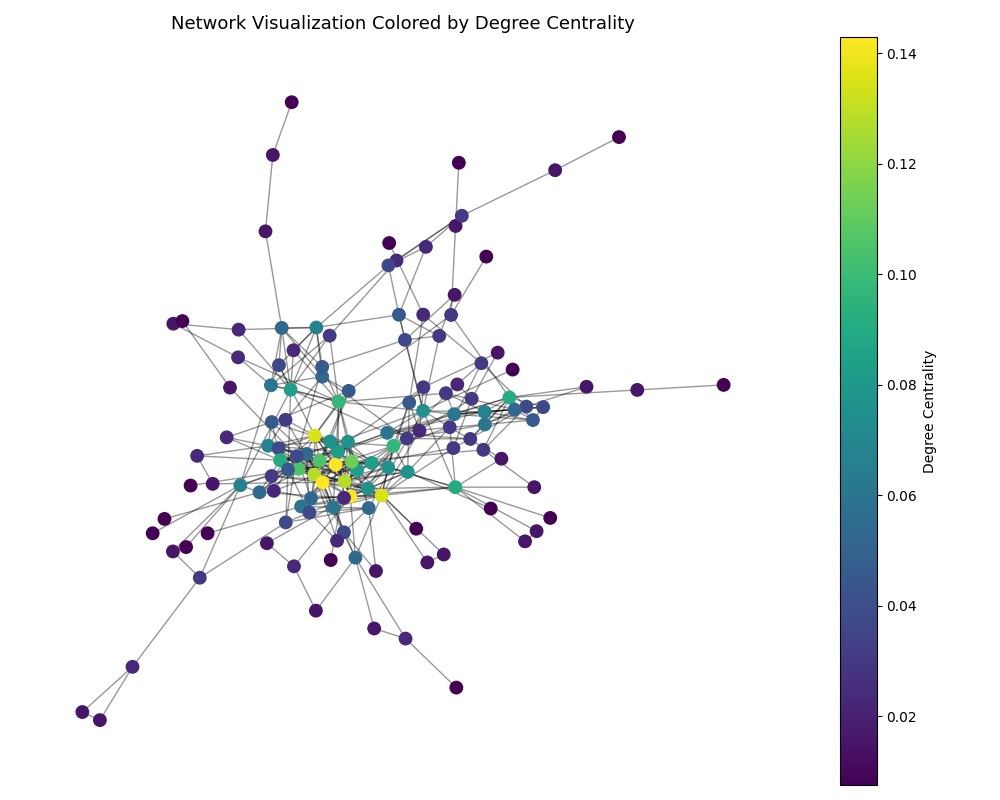
\includegraphics[width=0.8\textwidth]{Images/Centrality Measures.png}
    \caption{Network visualization colored by degree centrality.}
    \label{fig:centrality-visual}
\end{figure}

\section*{Interpretation}

The centrality analysis reveals several interesting insights:

\begin{itemize}
    \item Nodes 35, 38, and 54 have the highest degree centrality, suggesting they share burrows with many others—possibly because they frequent highly visited burrows or occupy overlapping territories.
    \item Node 61 stands out in betweenness centrality, despite not having high degree. This means it acts as a structural bridge connecting otherwise distant groups.
    \item Node 49, previously identified as the graph center, also has high betweenness, reinforcing its role in maintaining network cohesion.
    \item Nodes 38 and 54 consistently appear in the top 5 across all metrics, making them robust indicators of social centrality within the network.
\end{itemize}

These findings suggest that while most tortoises interact locally, a few play crucial roles in maintaining connectivity across the broader population.

% -- Degree Distribution --
\chapter*{Degree Distribution}
\addcontentsline{toc}{chapter}{Degree Distribution}

One of the most fundamental properties of a network is how its connections are distributed among nodes. This section explores the degree distribution of the tortoise network to assess whether certain individuals have disproportionately high numbers of interactions.

\section*{Degree Histogram}

Figure~\ref{fig:degree-histogram} shows the frequency distribution of node degrees. The histogram reveals a right-skewed pattern where most nodes have low degrees, but a few have significantly higher values.

\begin{figure}[h!]
    \centering
    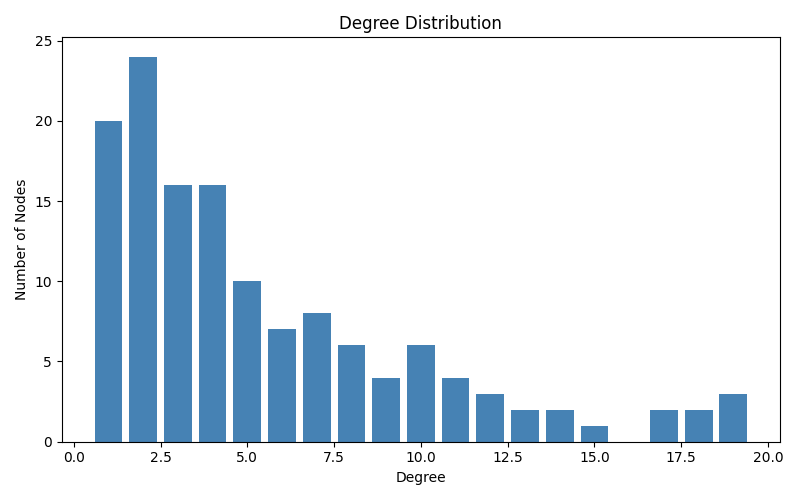
\includegraphics[width=0.75\textwidth]{Images/Degree Histogram.png}
    \caption{Histogram of node degrees in the tortoise network.}
    \label{fig:degree-histogram}
\end{figure}

\section*{Log-Log Distribution}

To determine whether the network follows a power-law (scale-free) distribution, a log-log plot was generated (Figure~\ref{fig:loglog-degree}).

\begin{figure}[h!]
    \centering
    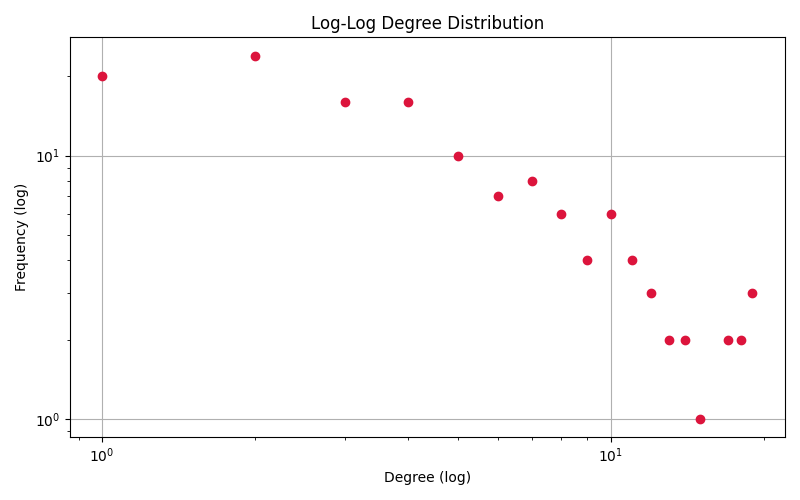
\includegraphics[width=0.75\textwidth]{Images/Log-Log Degree Distribution.png}
    \caption{Log-log plot of degree distribution.}
    \label{fig:loglog-degree}
\end{figure}

\section*{Summary Statistics}

\begin{itemize}
    \item Most common degree: 1 (20 nodes)
    \item Average degree: 5.50
    \item Minimum degree: 1
    \item Maximum degree: 19
\end{itemize}

\section*{Interpretation}

The degree distribution demonstrates a **heterogeneous structure**, where most tortoises share burrows with only a few others, and a minority function as local hubs. Although the log-log plot suggests a heavy-tailed distribution, it does not perfectly follow a straight line, implying the network is not strictly scale-free but still exhibits traits of **real-world social networks**.

This uneven connectivity could arise from:
\begin{itemize}
    \item Certain burrows being more frequently used or accessible
    \item Territorial overlap among specific individuals
    \item Behavioral differences such as higher movement or social tolerance
\end{itemize}

These patterns support the idea that the network is shaped by both ecological and spatial constraints, even in a species not typically viewed as social.

% -- Community Detection --
\chapter*{Community Detection}
\addcontentsline{toc}{chapter}{Community Detection}

To uncover potential substructures within the network, I applied the Louvain algorithm for community detection. This method partitions the graph by maximizing modularity, aiming to identify groups of nodes that are more densely connected internally than externally.

\section*{Results}

The algorithm identified \textbf{8 distinct communities} with a modularity score of \textbf{0.5568}, which is considered high and suggests a strong underlying community structure.

\begin{table}[h!]
    \centering
    \begin{tabular}{|c|c|}
        \hline
        \textbf{Community ID} & \textbf{Number of Nodes} \\\hline
        0 & 29 \\\hline
        1 & 10 \\\hline
        2 & 16 \\\hline
        3 & 19 \\\hline
        4 & 18 \\\hline
        5 & 13 \\\hline
        6 & 21 \\\hline
        7 & 8 \\\hline
        \textbf{Total} & \textbf{134 (LCC)} \\\hline
    \end{tabular}
    \caption{Detected communities and their sizes.}
    \label{tab:community-sizes}
\end{table}

\section*{Community Visualization}

Figure~\ref{fig:community-visual} shows the network colored by community assignment. The visualization reveals clearly defined clusters with a few nodes serving as bridges between them.

\begin{figure}[h!]
    \centering
    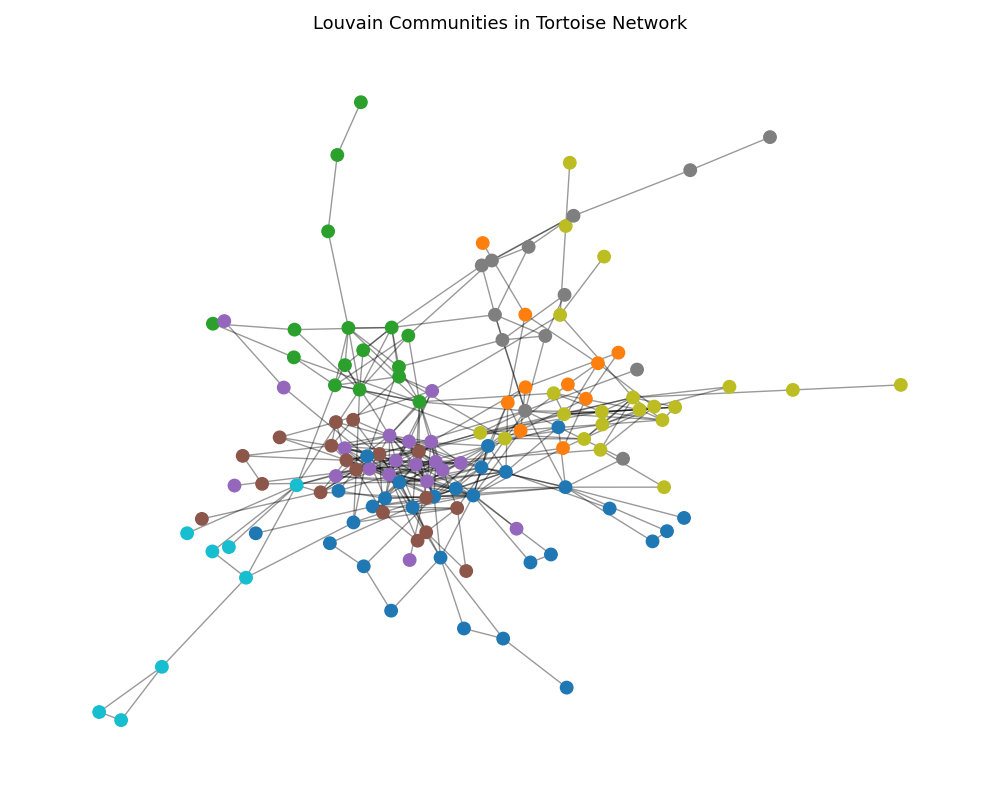
\includegraphics[width=0.8\textwidth]{Images/Community Detection.png}
    \caption{Communities detected using the Louvain algorithm.}
    \label{fig:community-visual}
\end{figure}

\section*{Interpretation}

The presence of eight well-separated communities confirms the network is not randomly structured. These communities likely correspond to tortoises with overlapping burrow usage patterns, influenced by spatial location and habitat availability. The relatively balanced sizes of each group (ranging from 8 to 29 nodes) suggest no dominant cluster exists, but rather a set of interconnected subgroups.

These patterns could reflect:
\begin{itemize}
    \item Geographic clustering around specific burrow zones
    \item Repeated use of shared refuges over time
    \item Potential temporal or seasonal overlap
\end{itemize}

The community structure aligns with observations from the degree and centrality analysis and reinforces the idea that even solitary animals can form implicit groupings through shared environmental use.

% -- Exploratory Conclusions & Temporal Dynamics --
\chapter*{Exploratory Conclusions \& Temporal Dynamics}
\addcontentsline{toc}{chapter}{Exploratory Conclusions \& Temporal Dynamics}

To complement the static analysis of the full network, I explored how the structure evolved over the four years of data collection (1996–1999), analyzing each year's snapshot individually.

\section*{Yearly Comparison Summary}

\begin{table}[h!]
    \centering
    \begin{tabular}{|c|c|c|c|c|c|c|}
        \hline
        \textbf{Year} & \textbf{Nodes} & \textbf{Edges} & \textbf{Density} & \textbf{Clustering} & \textbf{LCC Size} & \textbf{Diameter} \\\hline
        1996 & 12 & 7 & 0.1061 & 0.0000 & 4 & 3 \\\hline
        1997 & 105 & 189 & 0.0346 & 0.3561 & 94 & 13 \\\hline
        1998 & 89 & 191 & 0.0488 & 0.3378 & 82 & 13 \\\hline
        1999 & 69 & 105 & 0.0448 & 0.4123 & 33 & 13 \\\hline
    \end{tabular}
    \caption{Temporal network metrics per year.}
    \label{tab:temporal-comparison}
\end{table}

\section*{Interpretation}

The earliest year (1996) shows a small, fragmented network with no clustering, likely reflecting either low sampling or reduced tortoise activity. However, by 1997 and 1998, a large connected component emerges, along with moderate clustering values, suggesting stronger interaction zones formed by shared burrow use.

In 1999, the number of nodes drops and the largest component is smaller, yet clustering increases further. This may indicate that although interactions became more localized, they remained dense—possibly due to seasonal or spatial constraints.

These shifts suggest that the network structure is **dynamic** rather than stable, shaped over time by environmental conditions and tortoise behavior. While central individuals and communities exist, their prominence may vary depending on the year.

% -- Conclusion --
\chapter*{Conclusion}
\addcontentsline{toc}{chapter}{Conclusion}

This network analysis of the desert tortoise social structure, derived from shared refuge use, reveals a surprisingly organized and connected system for a species typically classified as solitary. The network exhibits key features of real-world social systems, including high clustering, centrality-rich nodes, and a clear community structure.

\begin{itemize}
    \item The network is sparse but highly clustered, with most individuals belonging to a single connected component.
    \item Centrality measures reveal both hubs (e.g., nodes 38, 54) and structural bridges (e.g., node 61).
    \item The degree distribution is heavy-tailed, suggesting social heterogeneity and spatial reuse patterns.
    \item Eight well-defined communities were detected, reinforcing the presence of localized groupings.
    \item Yearly snapshots confirm that the network structure evolves over time, with clustering increasing even as size fluctuates.
\end{itemize}

These findings challenge the assumption that solitary species lack social complexity. Instead, they demonstrate that interaction networks can emerge from indirect mechanisms such as shared habitat use. This study illustrates how tools from graph theory can provide valuable ecological insights and paves the way for further investigation into animal social systems using network science.

% -- References --
\chapter*{References}
\addcontentsline{toc}{chapter}{References}

\begin{itemize}
    \item Sah, P., Mann, J., \& Bansal, S. (2016). \textit{Inferring social structure and its drivers from refuge use in the desert tortoise, a relatively solitary species}. Behavioral Ecology and Sociobiology, 70(8), 1277–1289. https://doi.org/10.1007/s00265-016-2123-2

    \item Bansal Lab - Animal Social Network Repository. \textit{reptilia-tortoise-network-bsv}. Retrieved from: \texttt{https://bansallab.github.io/asnr/data.html}

    \item Hagberg, A., Schult, D., \& Swart, P. (2008). \textit{Exploring network structure, dynamics, and function using NetworkX}. In Proceedings of the 7th Python in Science Conference (SciPy2008), 11–15.
\end{itemize}



\end{document}